\section{Понятия реляционной теории}
\indent Для организации и теоретического обоснования описанного хранилища, использовалась теория реляционных баз данных.
\indent Теория реляционных баз данных оперирует понятиями отношения (relation, от которого и пошло само название теории и баз данных основанных на ней), атрибута, домена и кортежа.

\begin{figure}[ht]
	\centering
	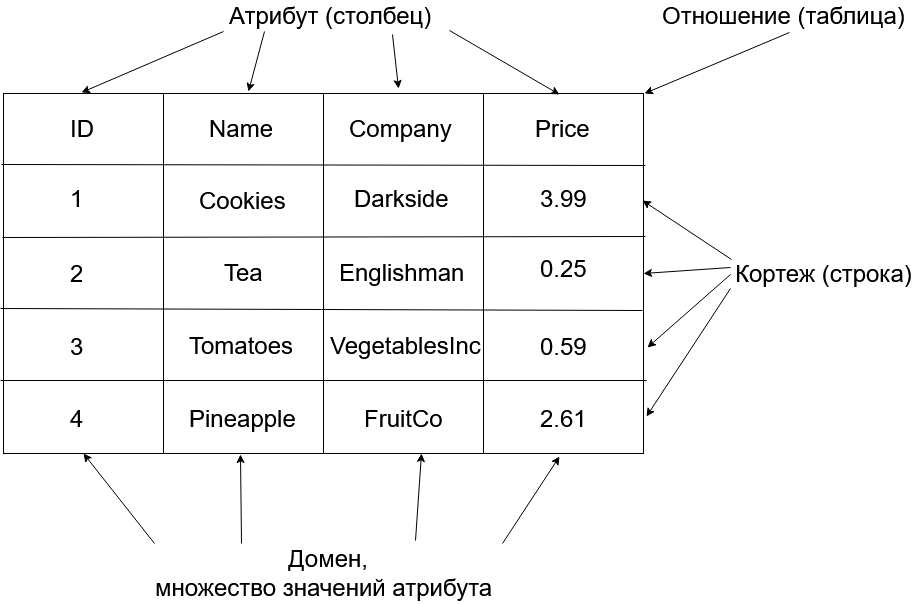
\includegraphics[width=\linewidth]{pics/databaseExample.png}
	\caption{Понятия реляционной базы данных}
	\label{fig:dbExample}
\end{figure}

\indent Атрибут -- именованный столбец отношения.
В пределах одного атрибута все значения должны быть одного типа данных, то есть принадлежать одному домену.\\
\indent Домен -- тип данных, множество всех допустимых значений атрибута.\\
\indent Кортеж -- упорядоченный набор из N элементов, где N -- это число атрибутов отношения.
Иначе говоря, кортеж -- это строка или запись таблицы.\\
\indent Отношение -- множество упорядоченных N-кортежей.
Другими словами отношение -- это двумерная (плоская) таблица, состоящая из столбцов и строк -- атрибутов и кортежей (см. рисунок \ref{fig:dbExample}).\\
\indent Также необходимо ввести понятие целостности по ссылкам заключающееся в отсутствии в любом её отношении внешних ключей (атрибут, указывающий на атрибут в другом отношении и совпадающий с ним по значению), ссылающихся на несуществующие кортежи.\\
\indent Так как любое отношение это множество, то им свойственны все операции определенные для множеств:
\begin{itemize}
	\item пересечение;
	\item объединение;
	\item вычитание;
	\item декартово произведение.
\end{itemize}
\indent Помимо этих четырех операций, в теории реляционной алгебры, вводится еще 4 операции свойственные только отношениям:
\begin{itemize}
	\item выборка ($\sigma_\phi(R)$) -- накладывает ограничение $\phi$ на отношение $R$;
	\item проекция ($\pi_\phi(R)$) -- отображает только те атрибуты отношения $R$, которые были представлены в $\phi$;
	\item соединение ($R_1\ \bowtie_\phi\ R_2$) -- соединяет кортежи из двух отношений $R_1$ и $R_2$ по условию $\phi$;
	\item переименование ($\rho_{a,b}(R)$) -- переименовывает атрибут отношения $R$ из $a$ в $b$ .
\end{itemize}
\todo[inline]{дать определения операциям над множествами}